\section{Validation}
\subsection{Comparison of inbending and outbending data}
One of the validation tests performed on our data is to see if the results are independent of the torus-field polarity.  The first stage of this test is to select only events in the region of overlap between the two configurations.  For the data with the in-bending (out-bending) configuration, particles with positive (negative) charge can be observed at smaller polar angles\footnote{at the interaction point} than in out-bending (in-bending) configuration.  This is demonstrated in Figs.~\ref{fig:p_vs_th_inout_e}, \ref{fig:p_vs_th_inout_h1} and \ref{fig:p_vs_th_inout_h2}, which contain $p$ vs $\theta$ scatter plots of the in-bending (blue) and out-bending (orange) datasets (respectively  for $e$,$h_1$ and $h_2$).  Each of the panels shows a different configuration of hadron types.    

\begin{figure}
    \centering
    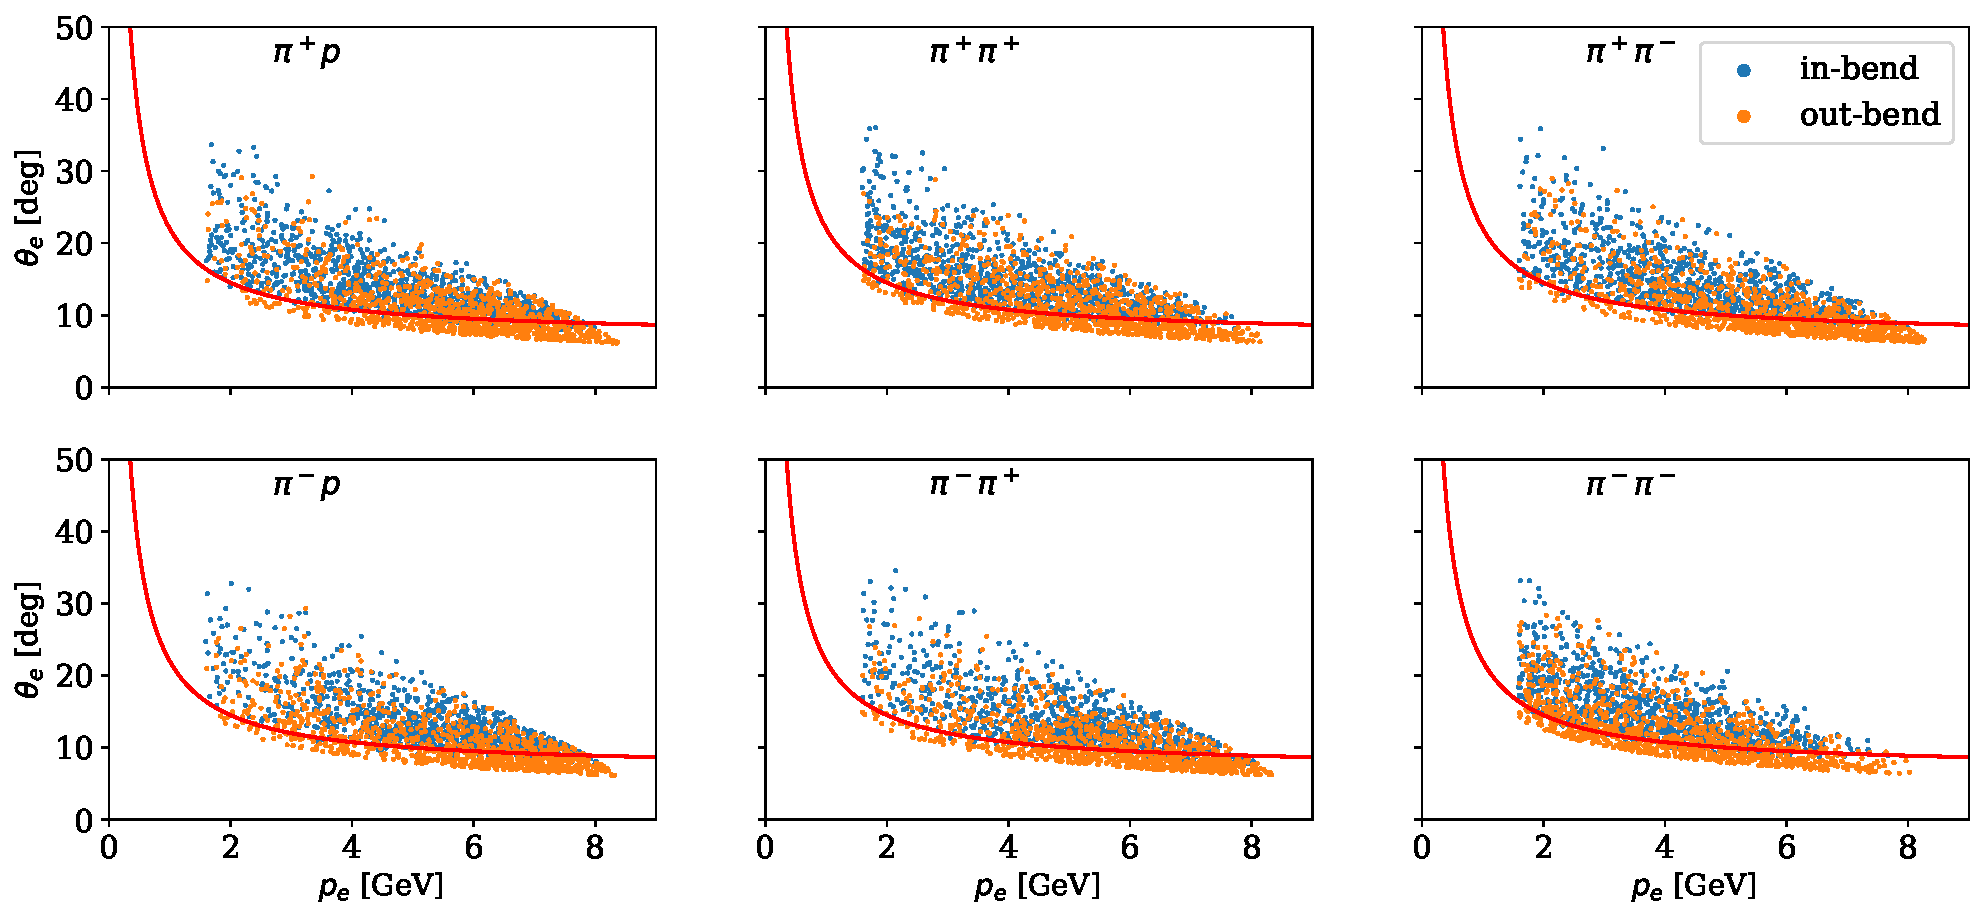
\includegraphics[width=\textwidth]{images/p_vs_th_inout_e.pdf}
    \caption{Electron momentum vs polar angle spectra (lab frame) for data in the in-bending (blue) and out-bending (orange) torus configurations.  The different panels represent different configurations of  di-hadron types.}
    \label{fig:p_vs_th_inout_e}
\end{figure}

\begin{figure}
    \centering
    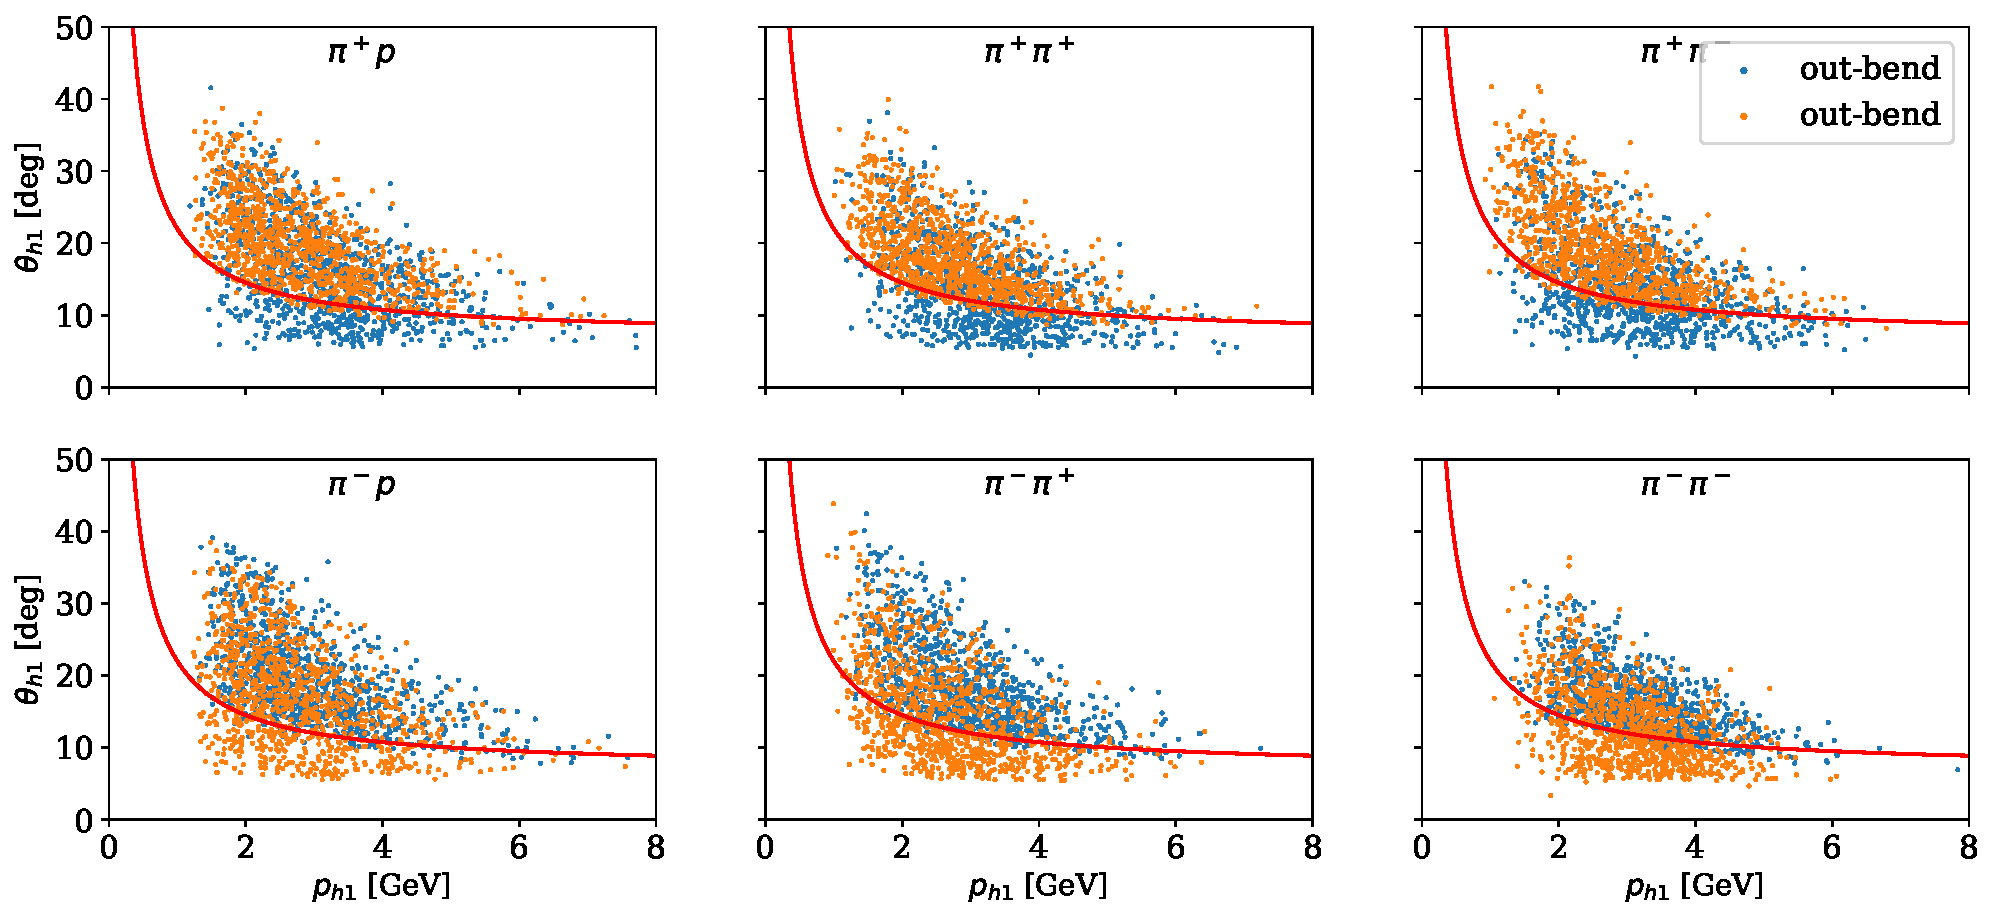
\includegraphics[width=\textwidth]{images/p_vs_th_inout_h1.pdf}
    \caption{Same as Fig.~\ref{fig:p_vs_th_inout_e} for the leading hadron's momentum and polar angle.}
    \label{fig:p_vs_th_inout_h1}
\end{figure}

\begin{figure}
    \centering
    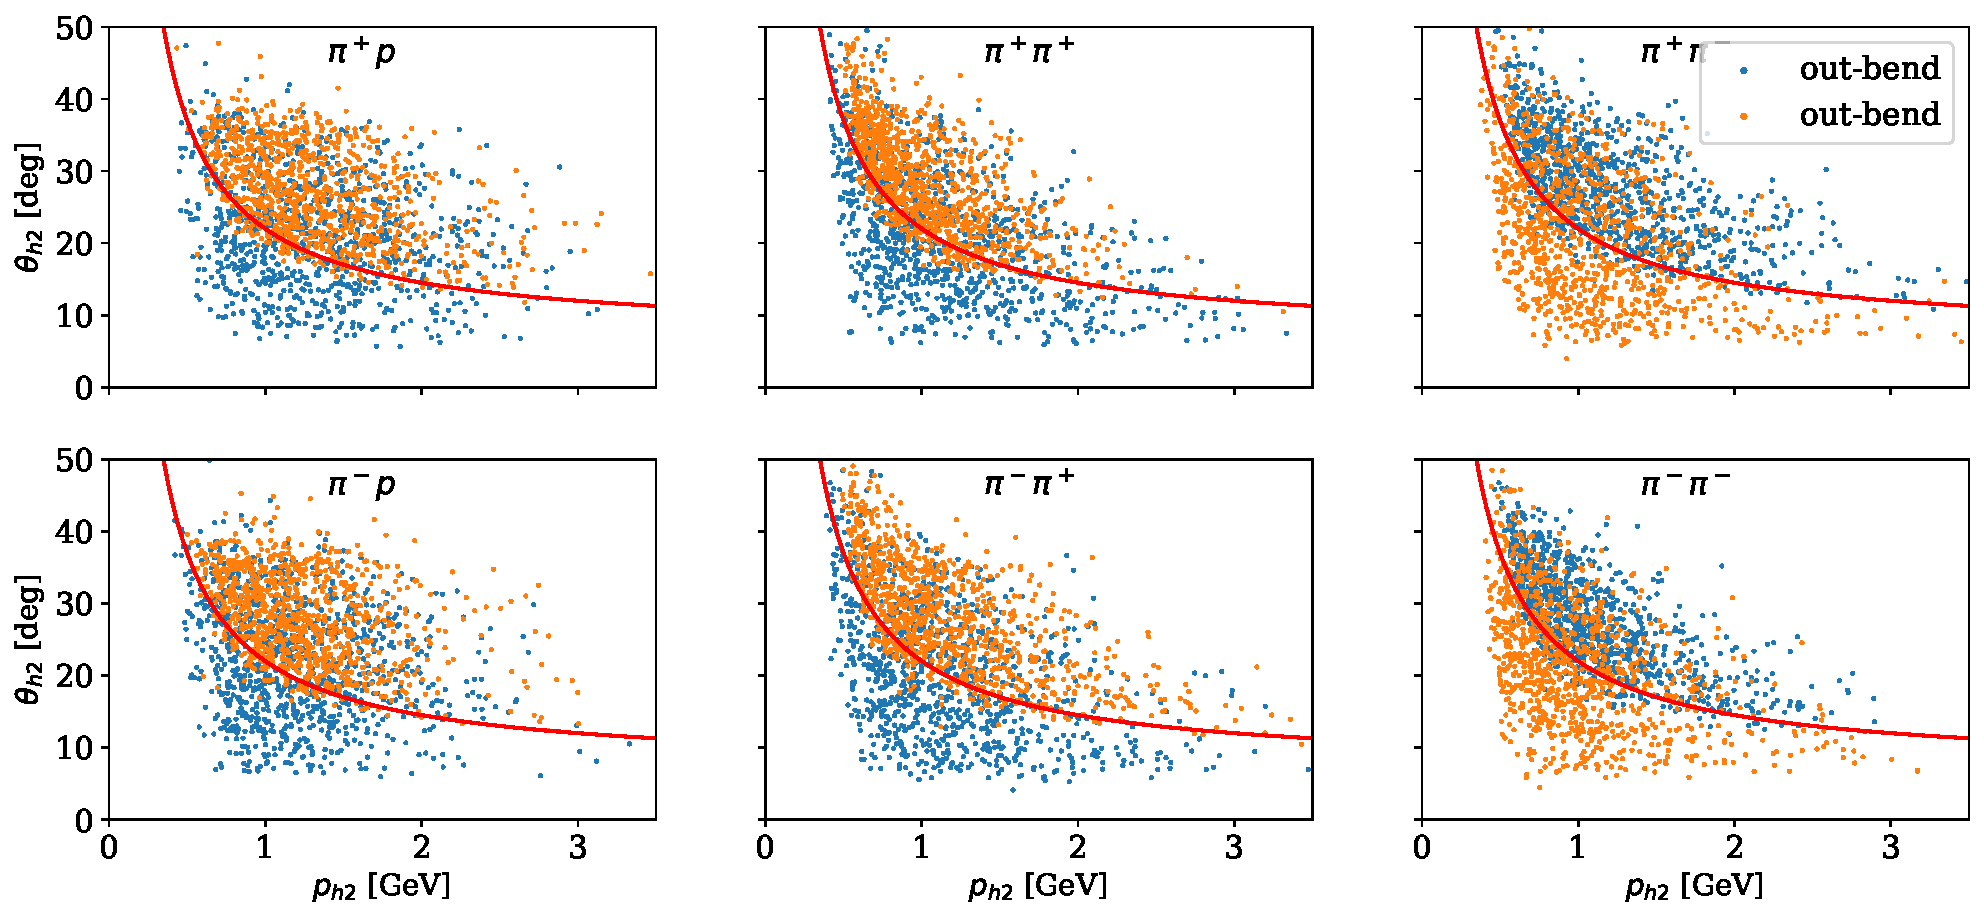
\includegraphics[width=\textwidth]{images/p_vs_th_inout_h2.pdf}
    \caption{Same as Fig.~\ref{fig:p_vs_th_inout_e} for the sub-leading hadron's momentum and polar angle.}
    \label{fig:p_vs_th_inout_h2}
\end{figure}

In order to only include events in the kinematic region where the data taken with the two field polarities overlap, we used following kinematic cuts on each of the three particles ($e$,$h_1$ and $h_2$):
\begin{equation}
    \theta > 7\degree + \frac{15\degree}{p/{\rm GeV}}
\end{equation}
where $p$ and $\theta$ are the lab-frame momenta and polar angles for the particle.  This is shown as a red line in Figs.~\ref{fig:p_vs_th_inout_e}-\ref{fig:p_vs_th_inout_h2}.   



Figs.~\ref{fig:smc_inout_pi+p} through~\ref{fig:smc_inout_pi-pi-} shows the same-event yields, mixed-event yields and correlation functions for each combination of particle observed ($\pi^+ p$, $\pi^- p$, $\pi^+\pi^+$, $\pi^-\pi^+$, $\pi^+\pi^-$ and $\pi^+\pi^-$). The top (middle) row panel of each figure shows the 2d functions for in-bending (out-bending) data.  The bottom rows show the 1d projections in the $\Delta y=1.5$ to 2.5 range, with in-bending (out-bending) data in blue (orange).  

\begin{figure}
    \centering
    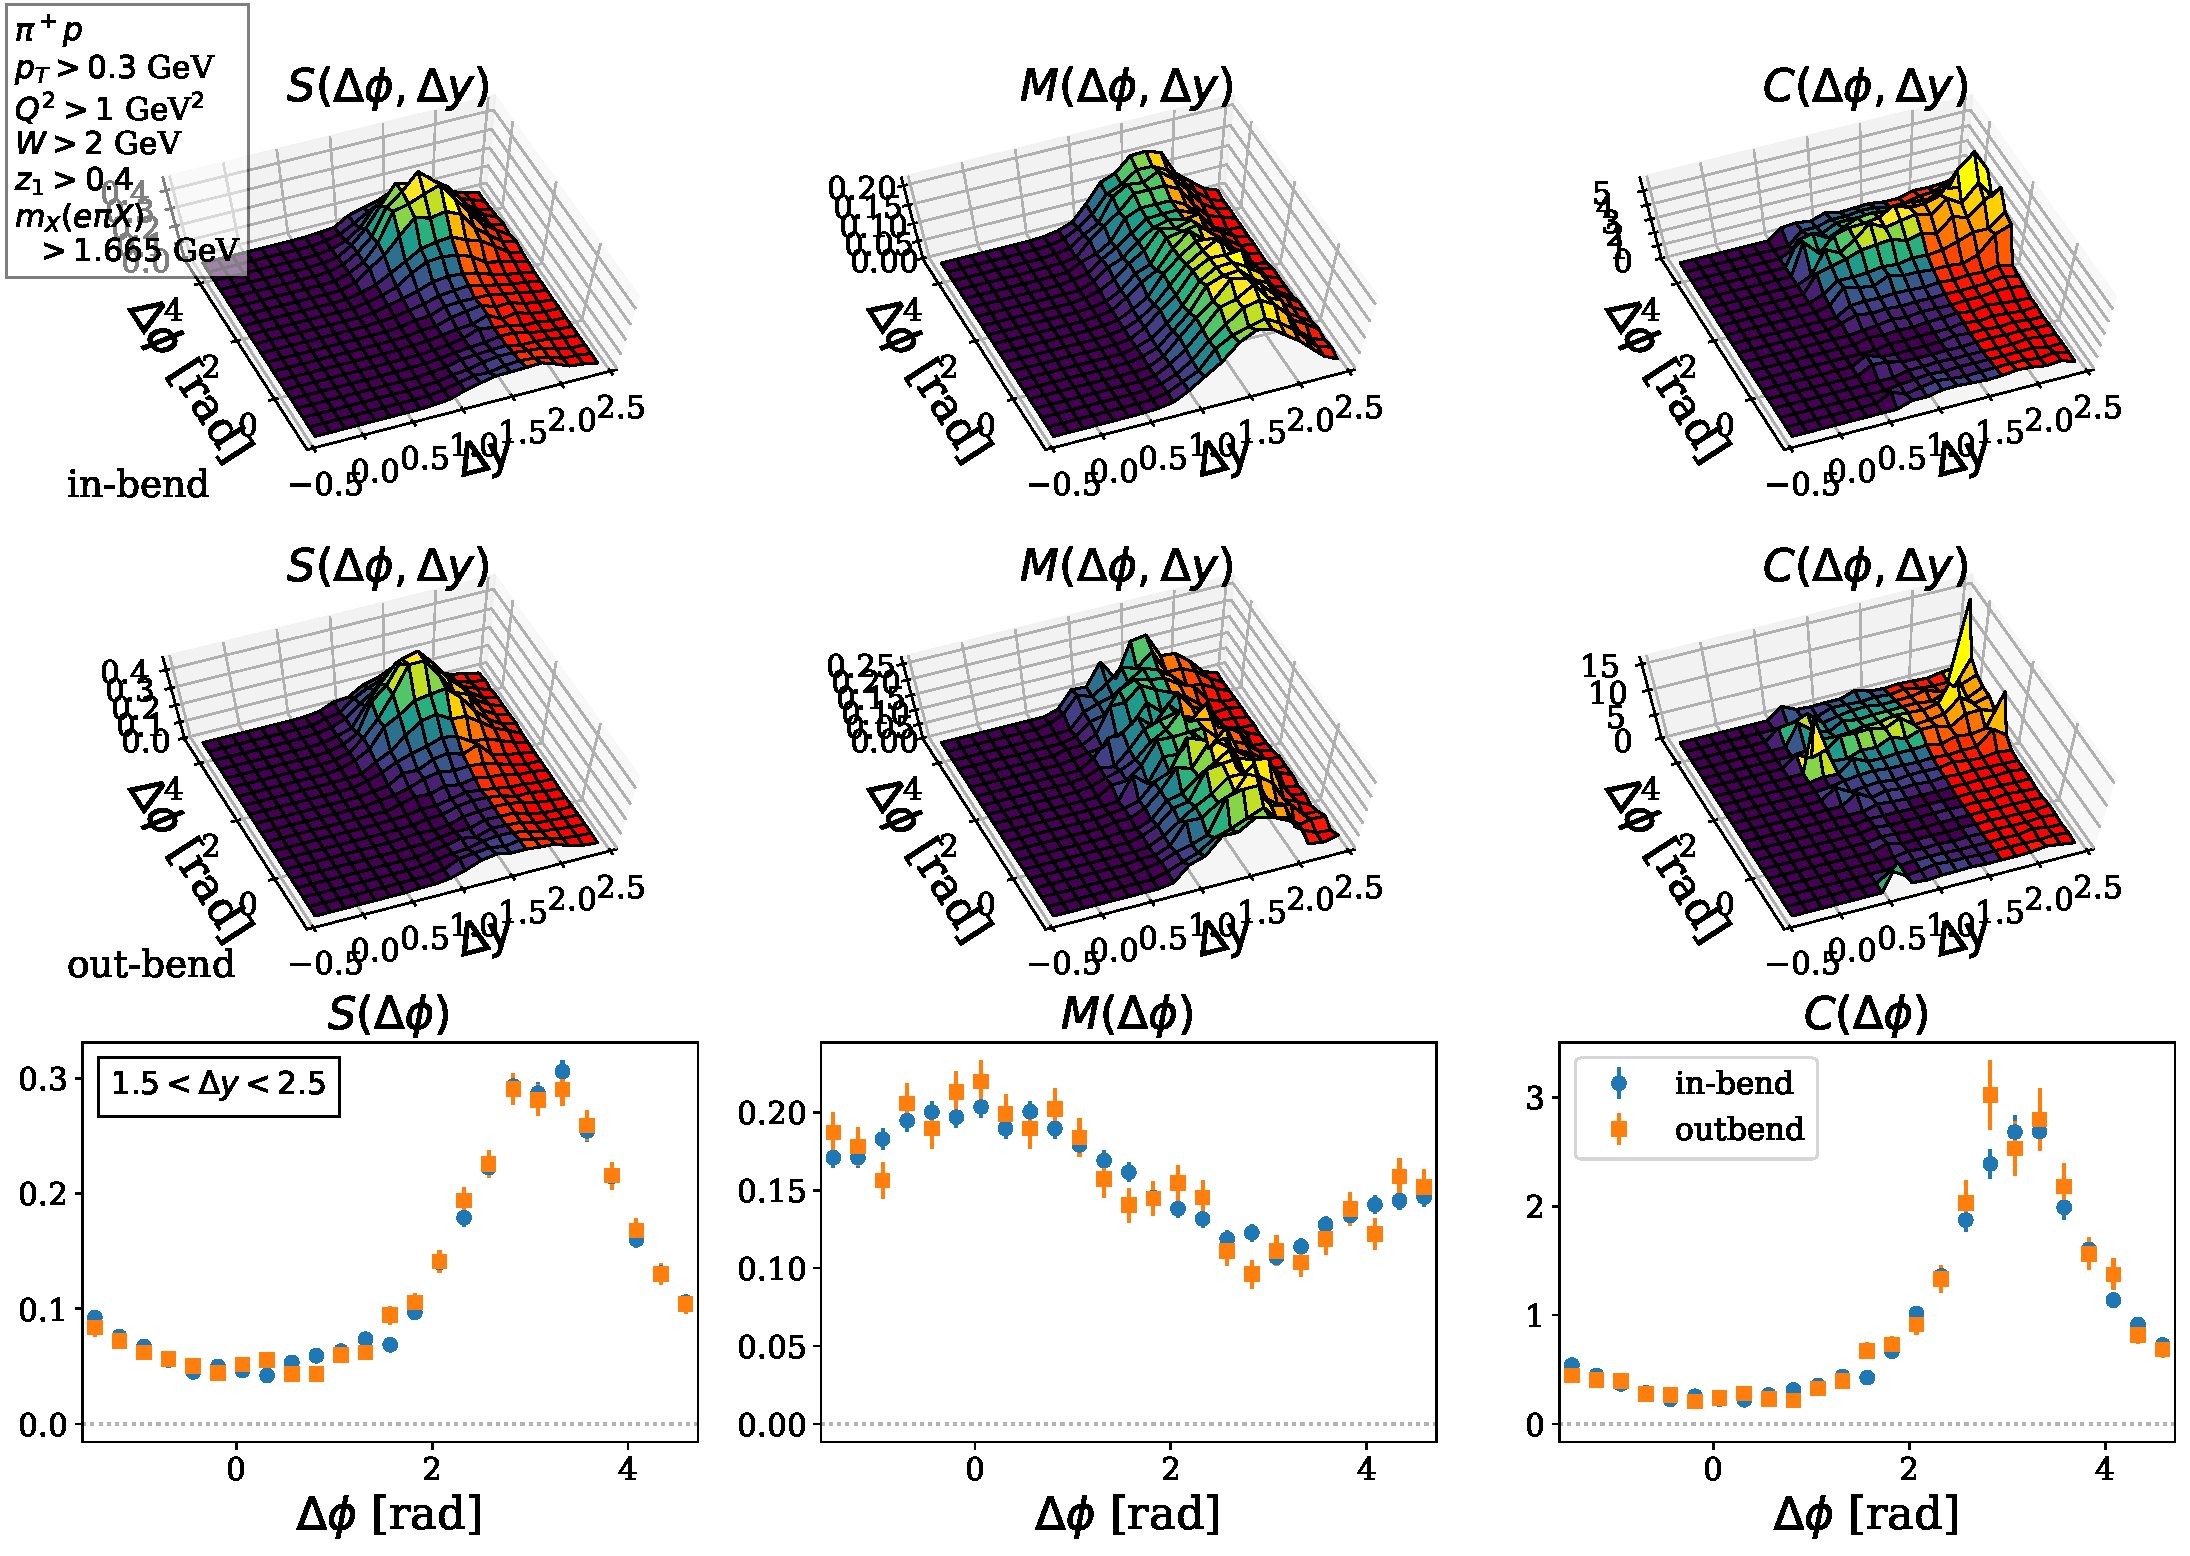
\includegraphics[width=\textwidth]{images/smc_inout_pi+p.pdf}
    \caption{Comparison of same-event yields (left column), mixed-event yields (middle column), and correlation functions (right column) for in-bending and out-bending data for $\pi^+ p$.  The top (middle) row shows the 2d functions for in-bending (out-bending) data.  The bottom row shows the 1d projections in the $\Delta y=1.5$ to 2.5 range, with in-bending (out-bending) data in blue (orange).}
    \label{fig:smc_inout_pi+p}
\end{figure}

\begin{figure}
    \centering
    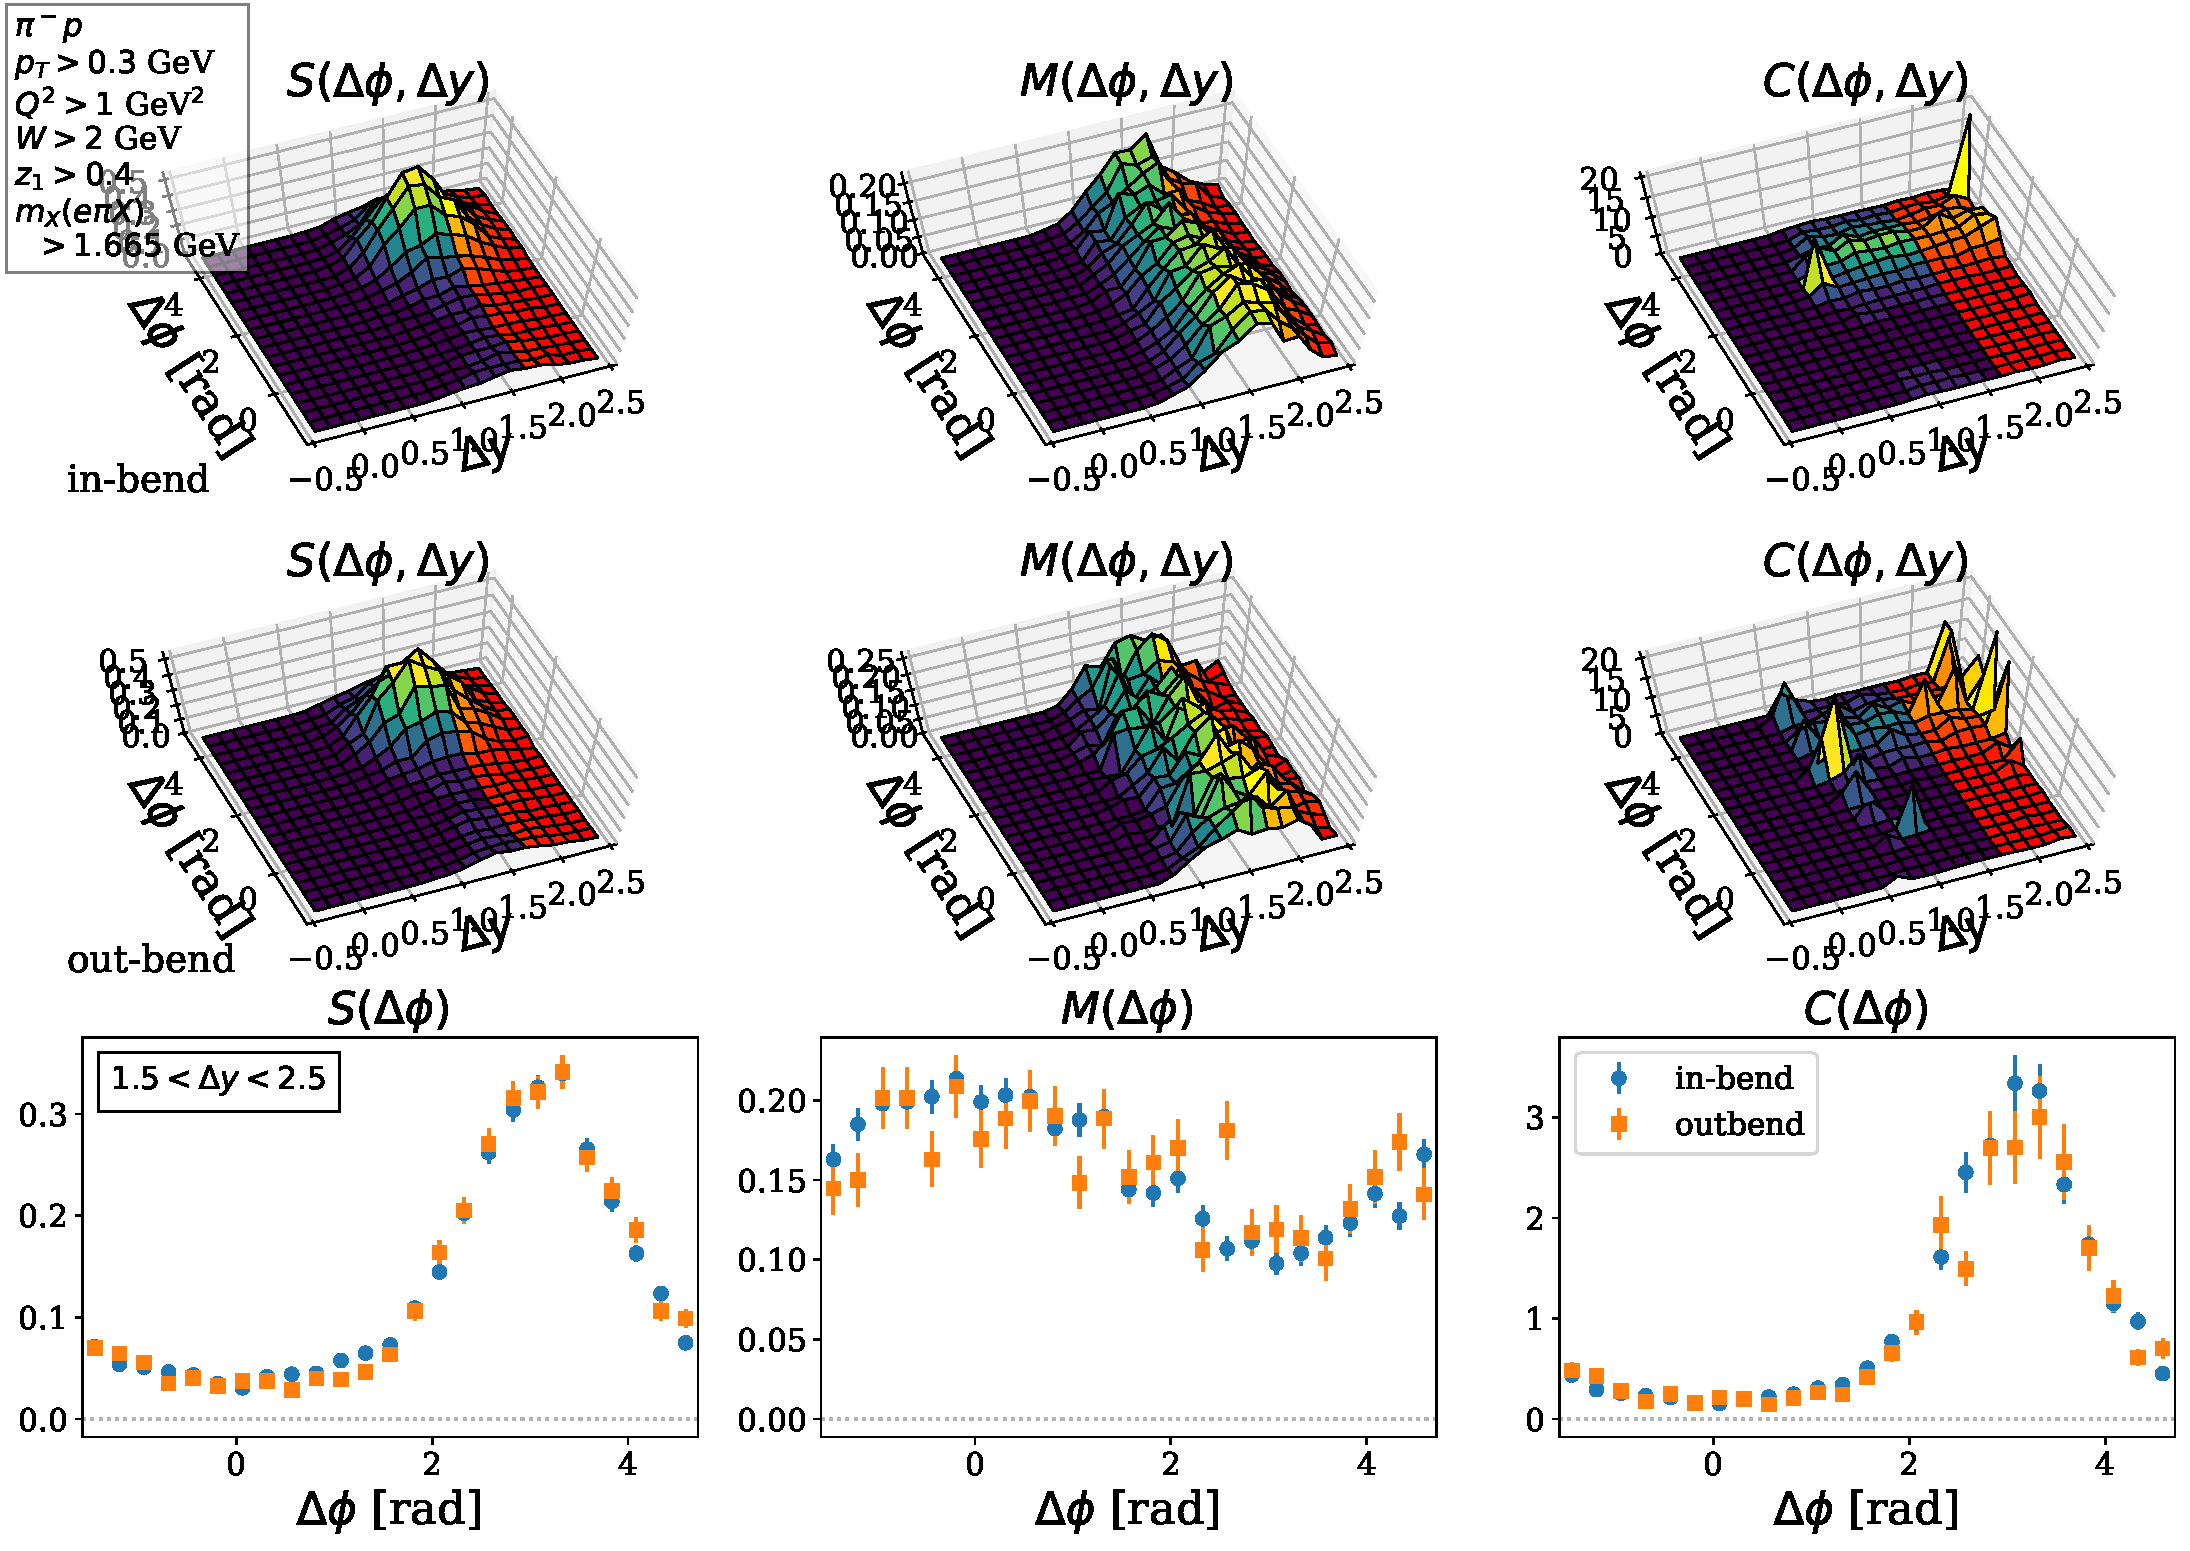
\includegraphics[width=\textwidth]{images/smc_inout_pi-p.pdf}
    \caption{Same as Fig.~\ref{fig:smc_inout_pi+p} for $\pi^- p$}
    \label{fig:smc_inout_pi-p}
\end{figure}

\begin{figure}
    \centering
    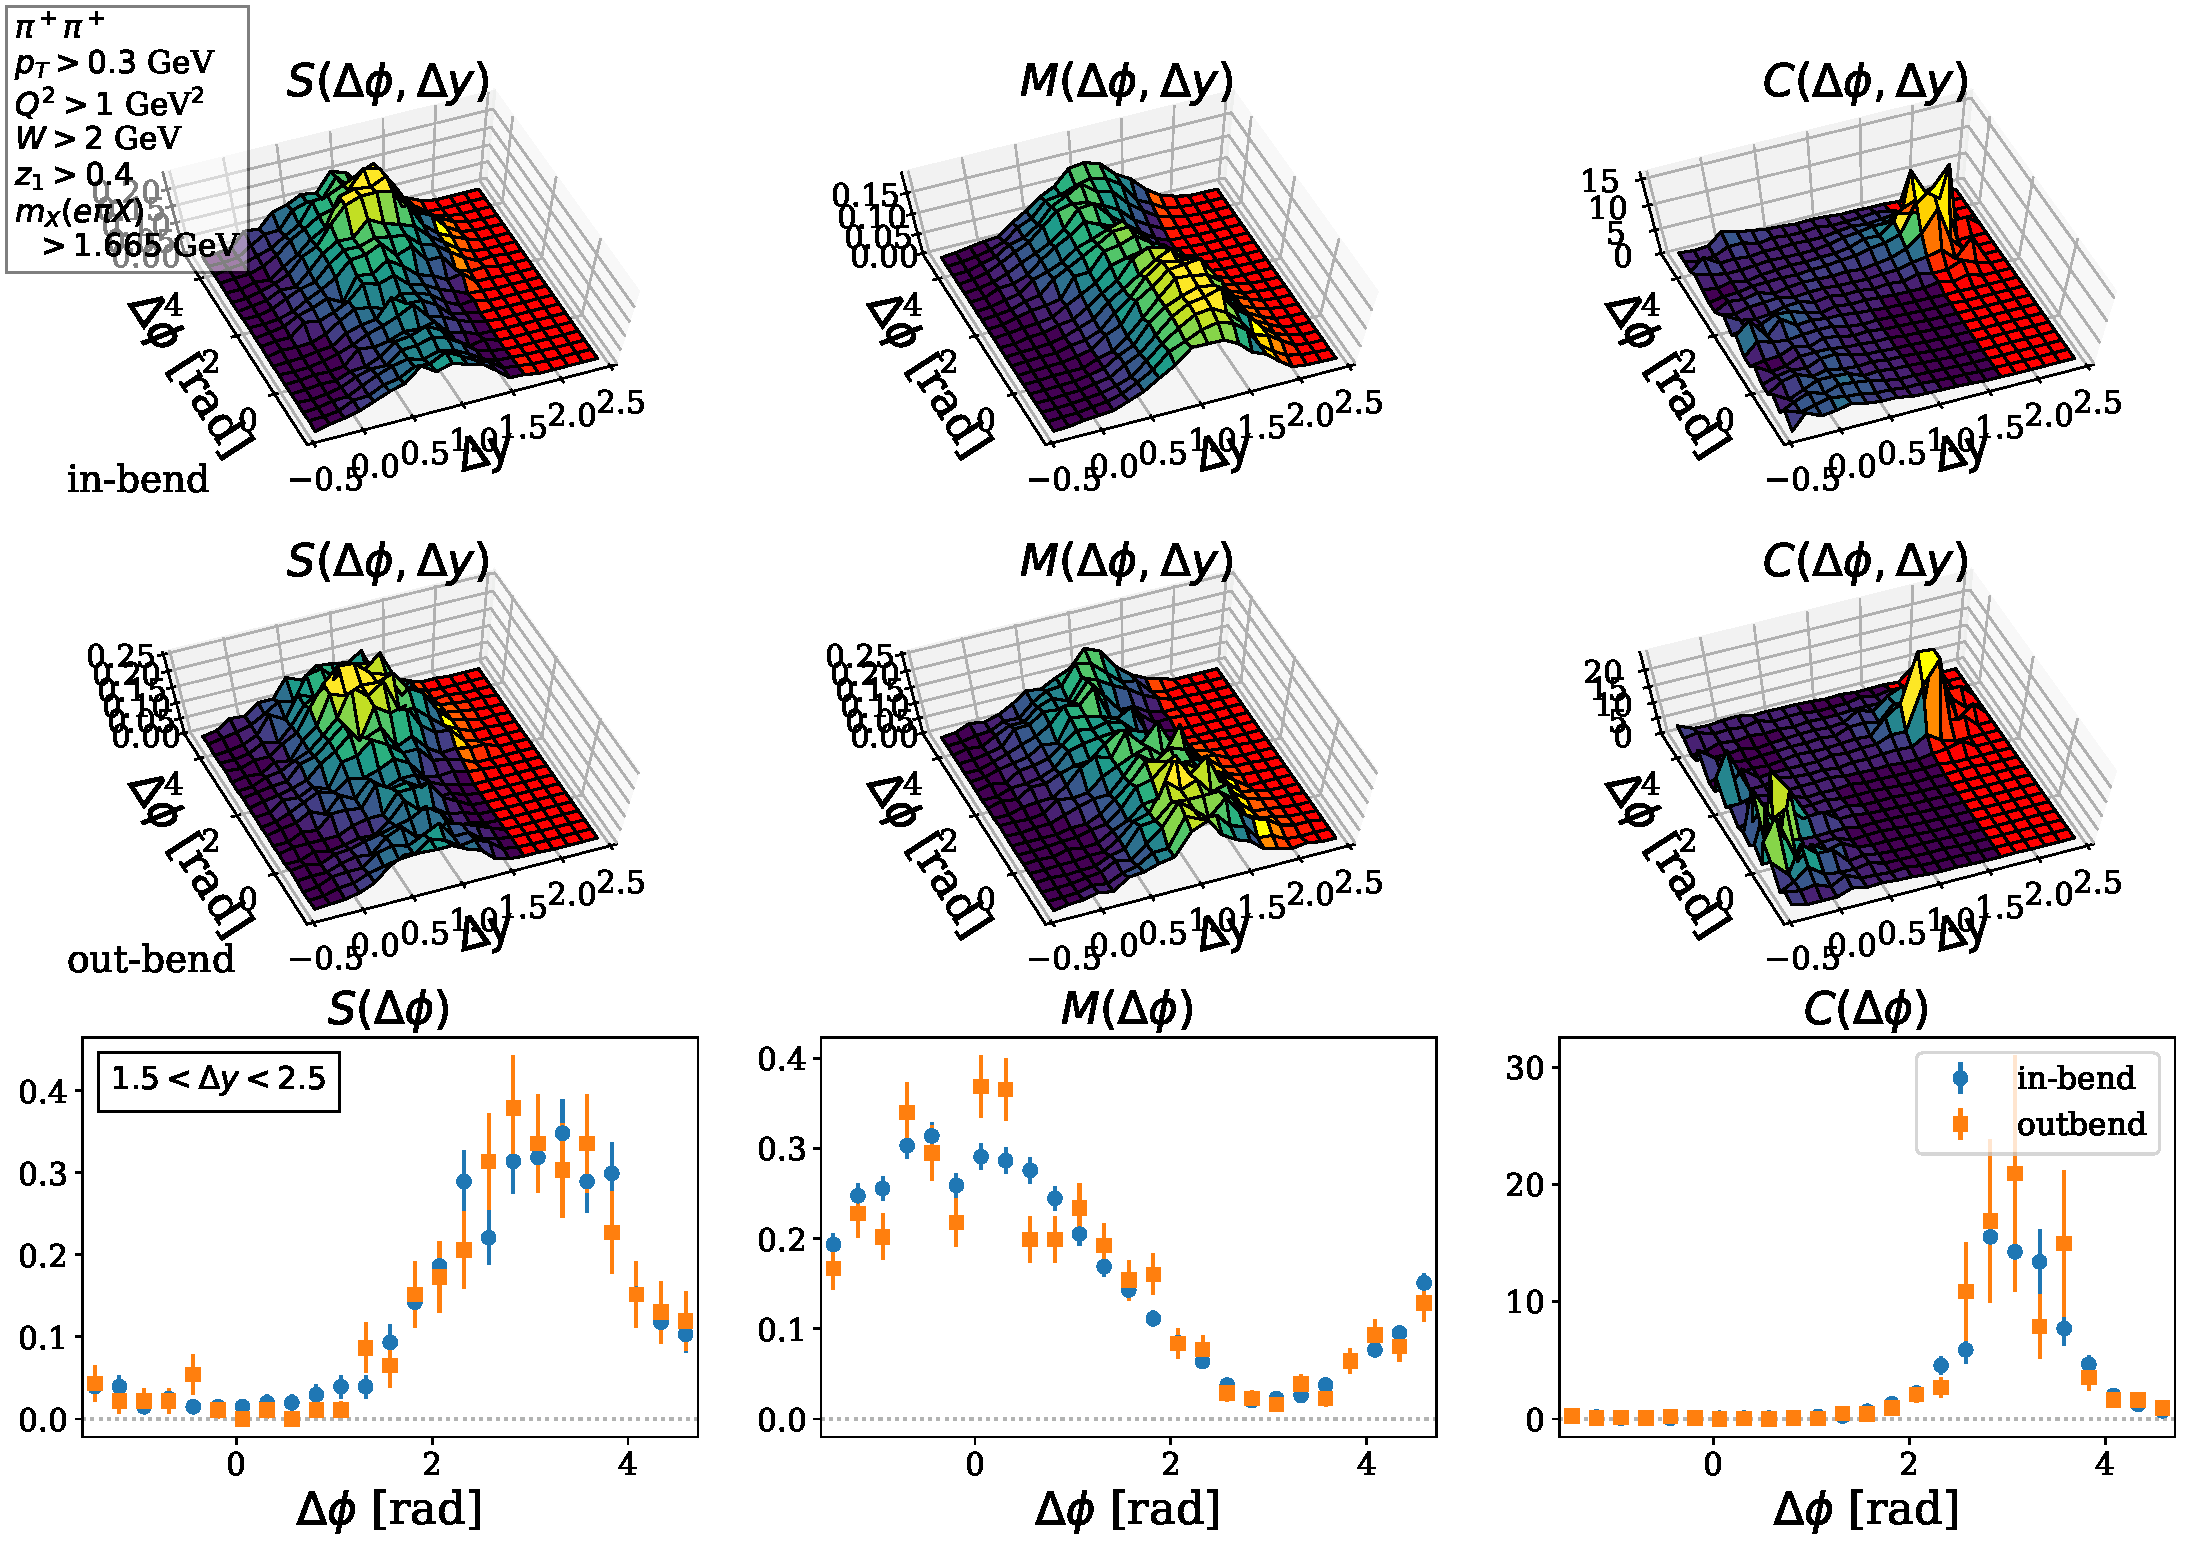
\includegraphics[width=\textwidth]{images/smc_inout_pi+pi+.pdf}
    \caption{Same as Fig.~\ref{fig:smc_inout_pi+p} for $\pi^+\pi^+$}
    \label{fig:smc_inout_pi+pi+}
\end{figure}

\begin{figure}
    \centering
    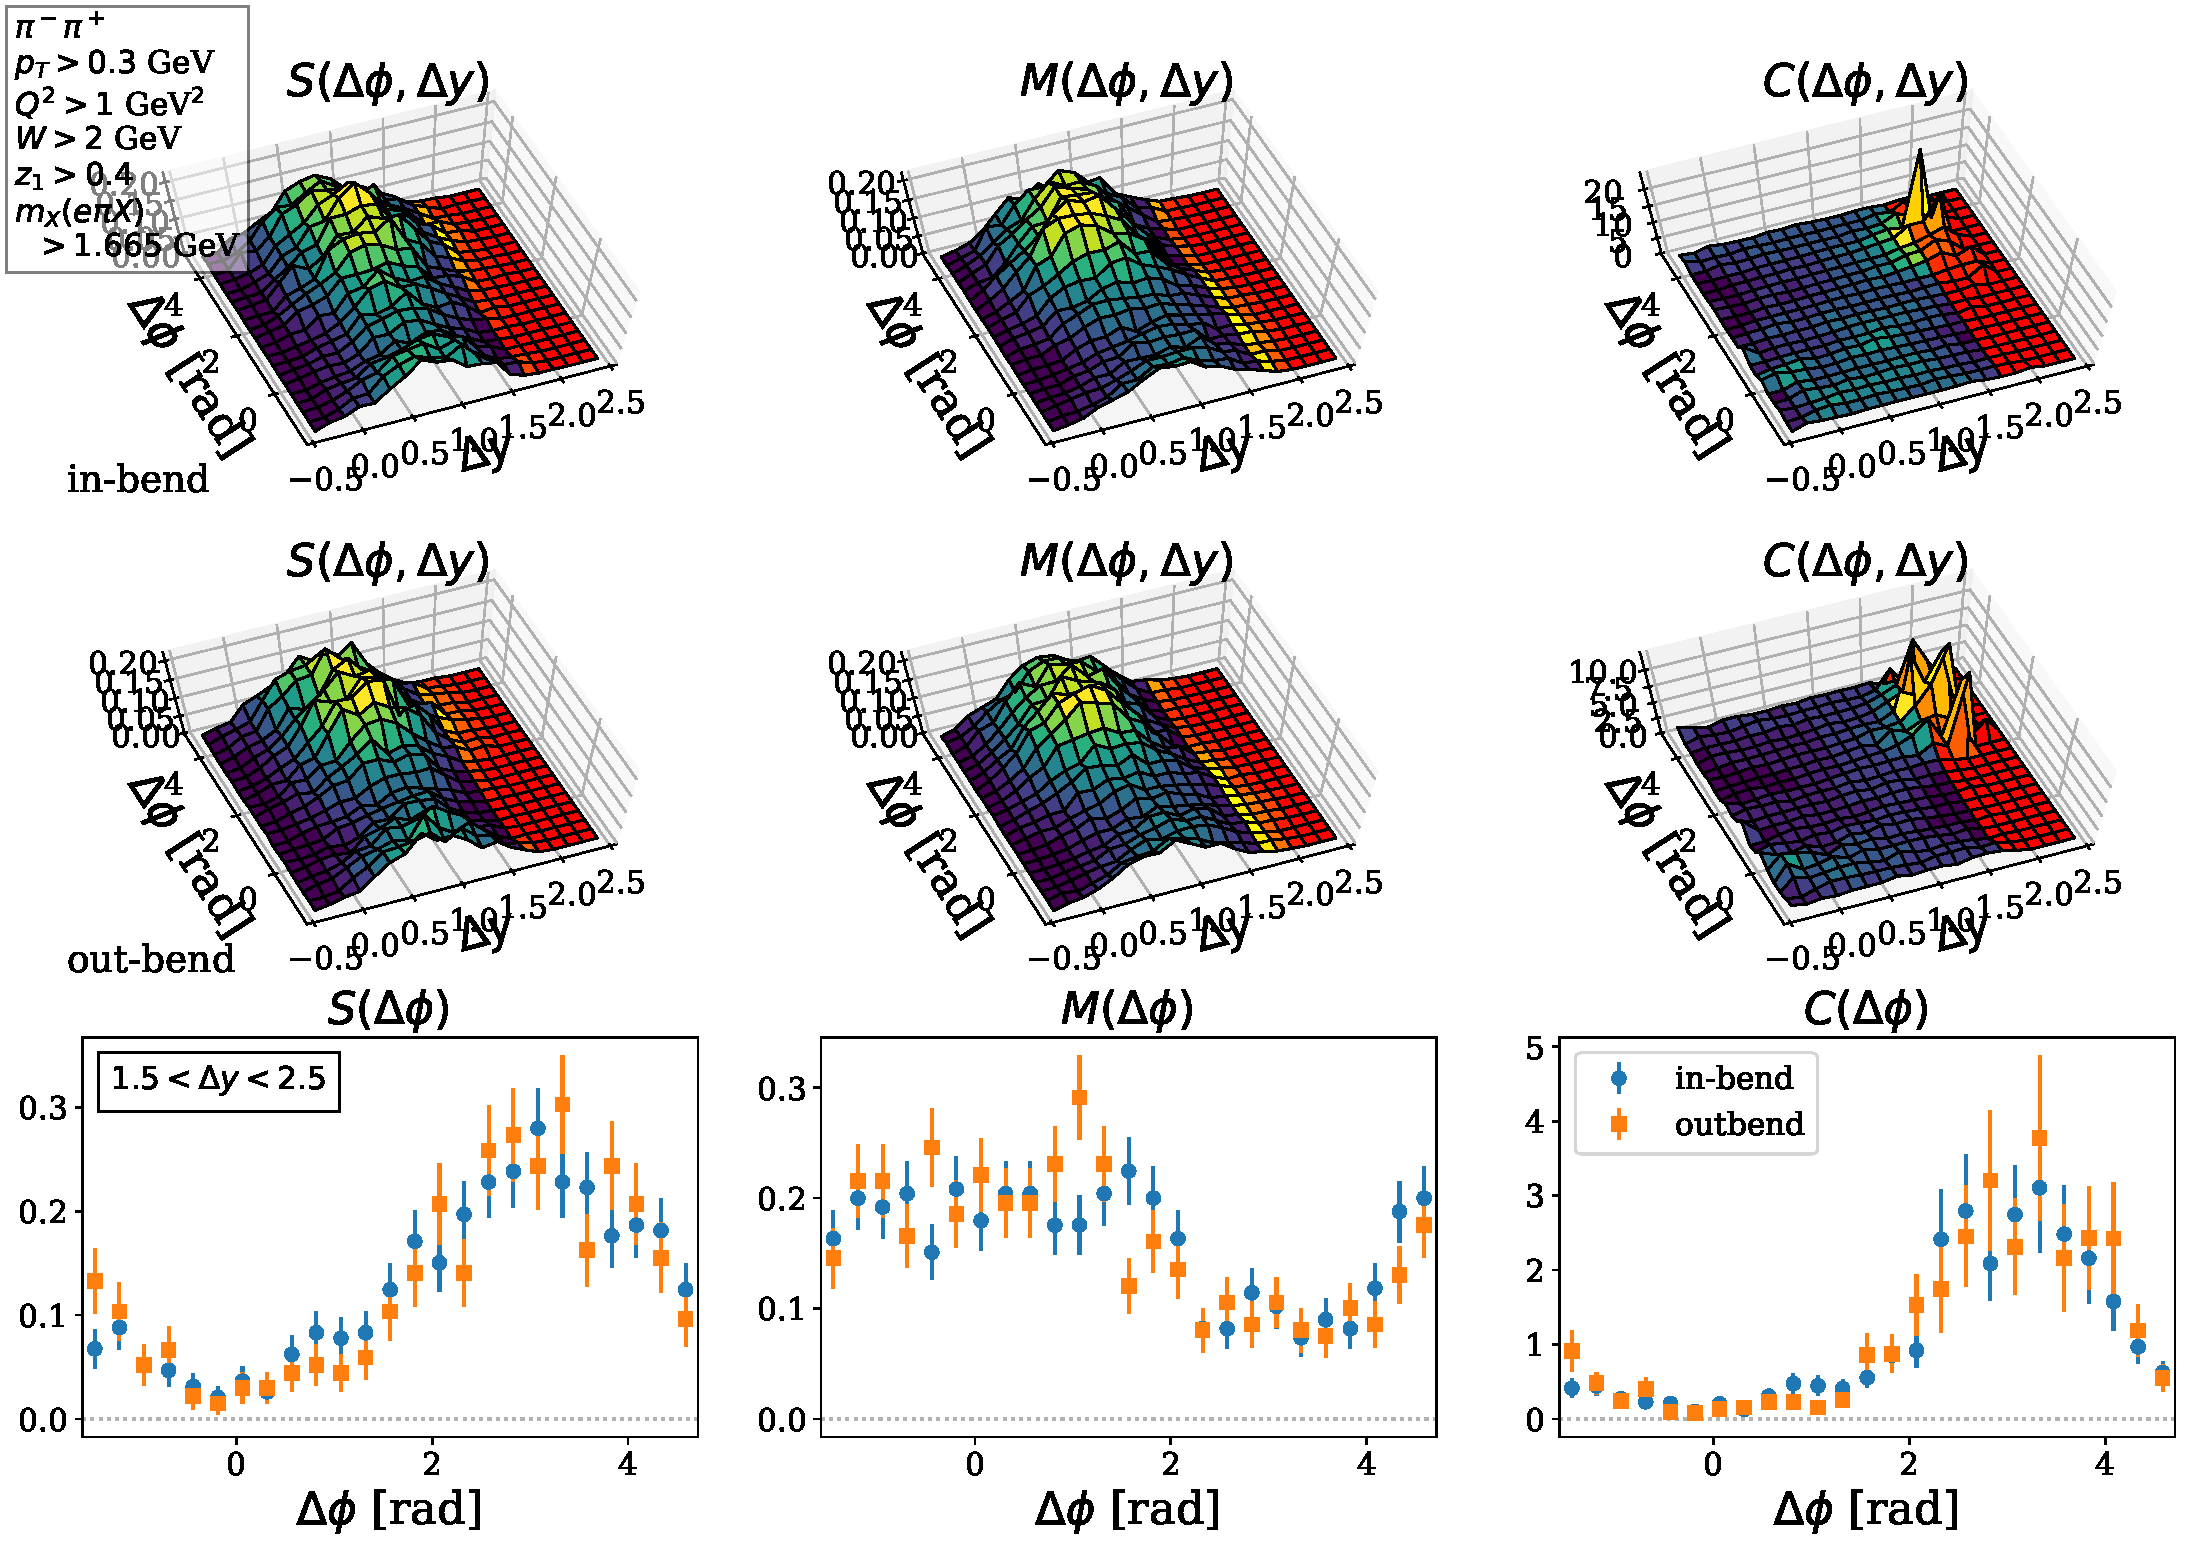
\includegraphics[width=\textwidth]{images/smc_inout_pi-pi+.pdf}
    \caption{Same as Fig.~\ref{fig:smc_inout_pi+p} for $\pi^-\pi^+$}
    \label{fig:smc_inout_pi-pi+}
\end{figure}

\begin{figure}
    \centering
    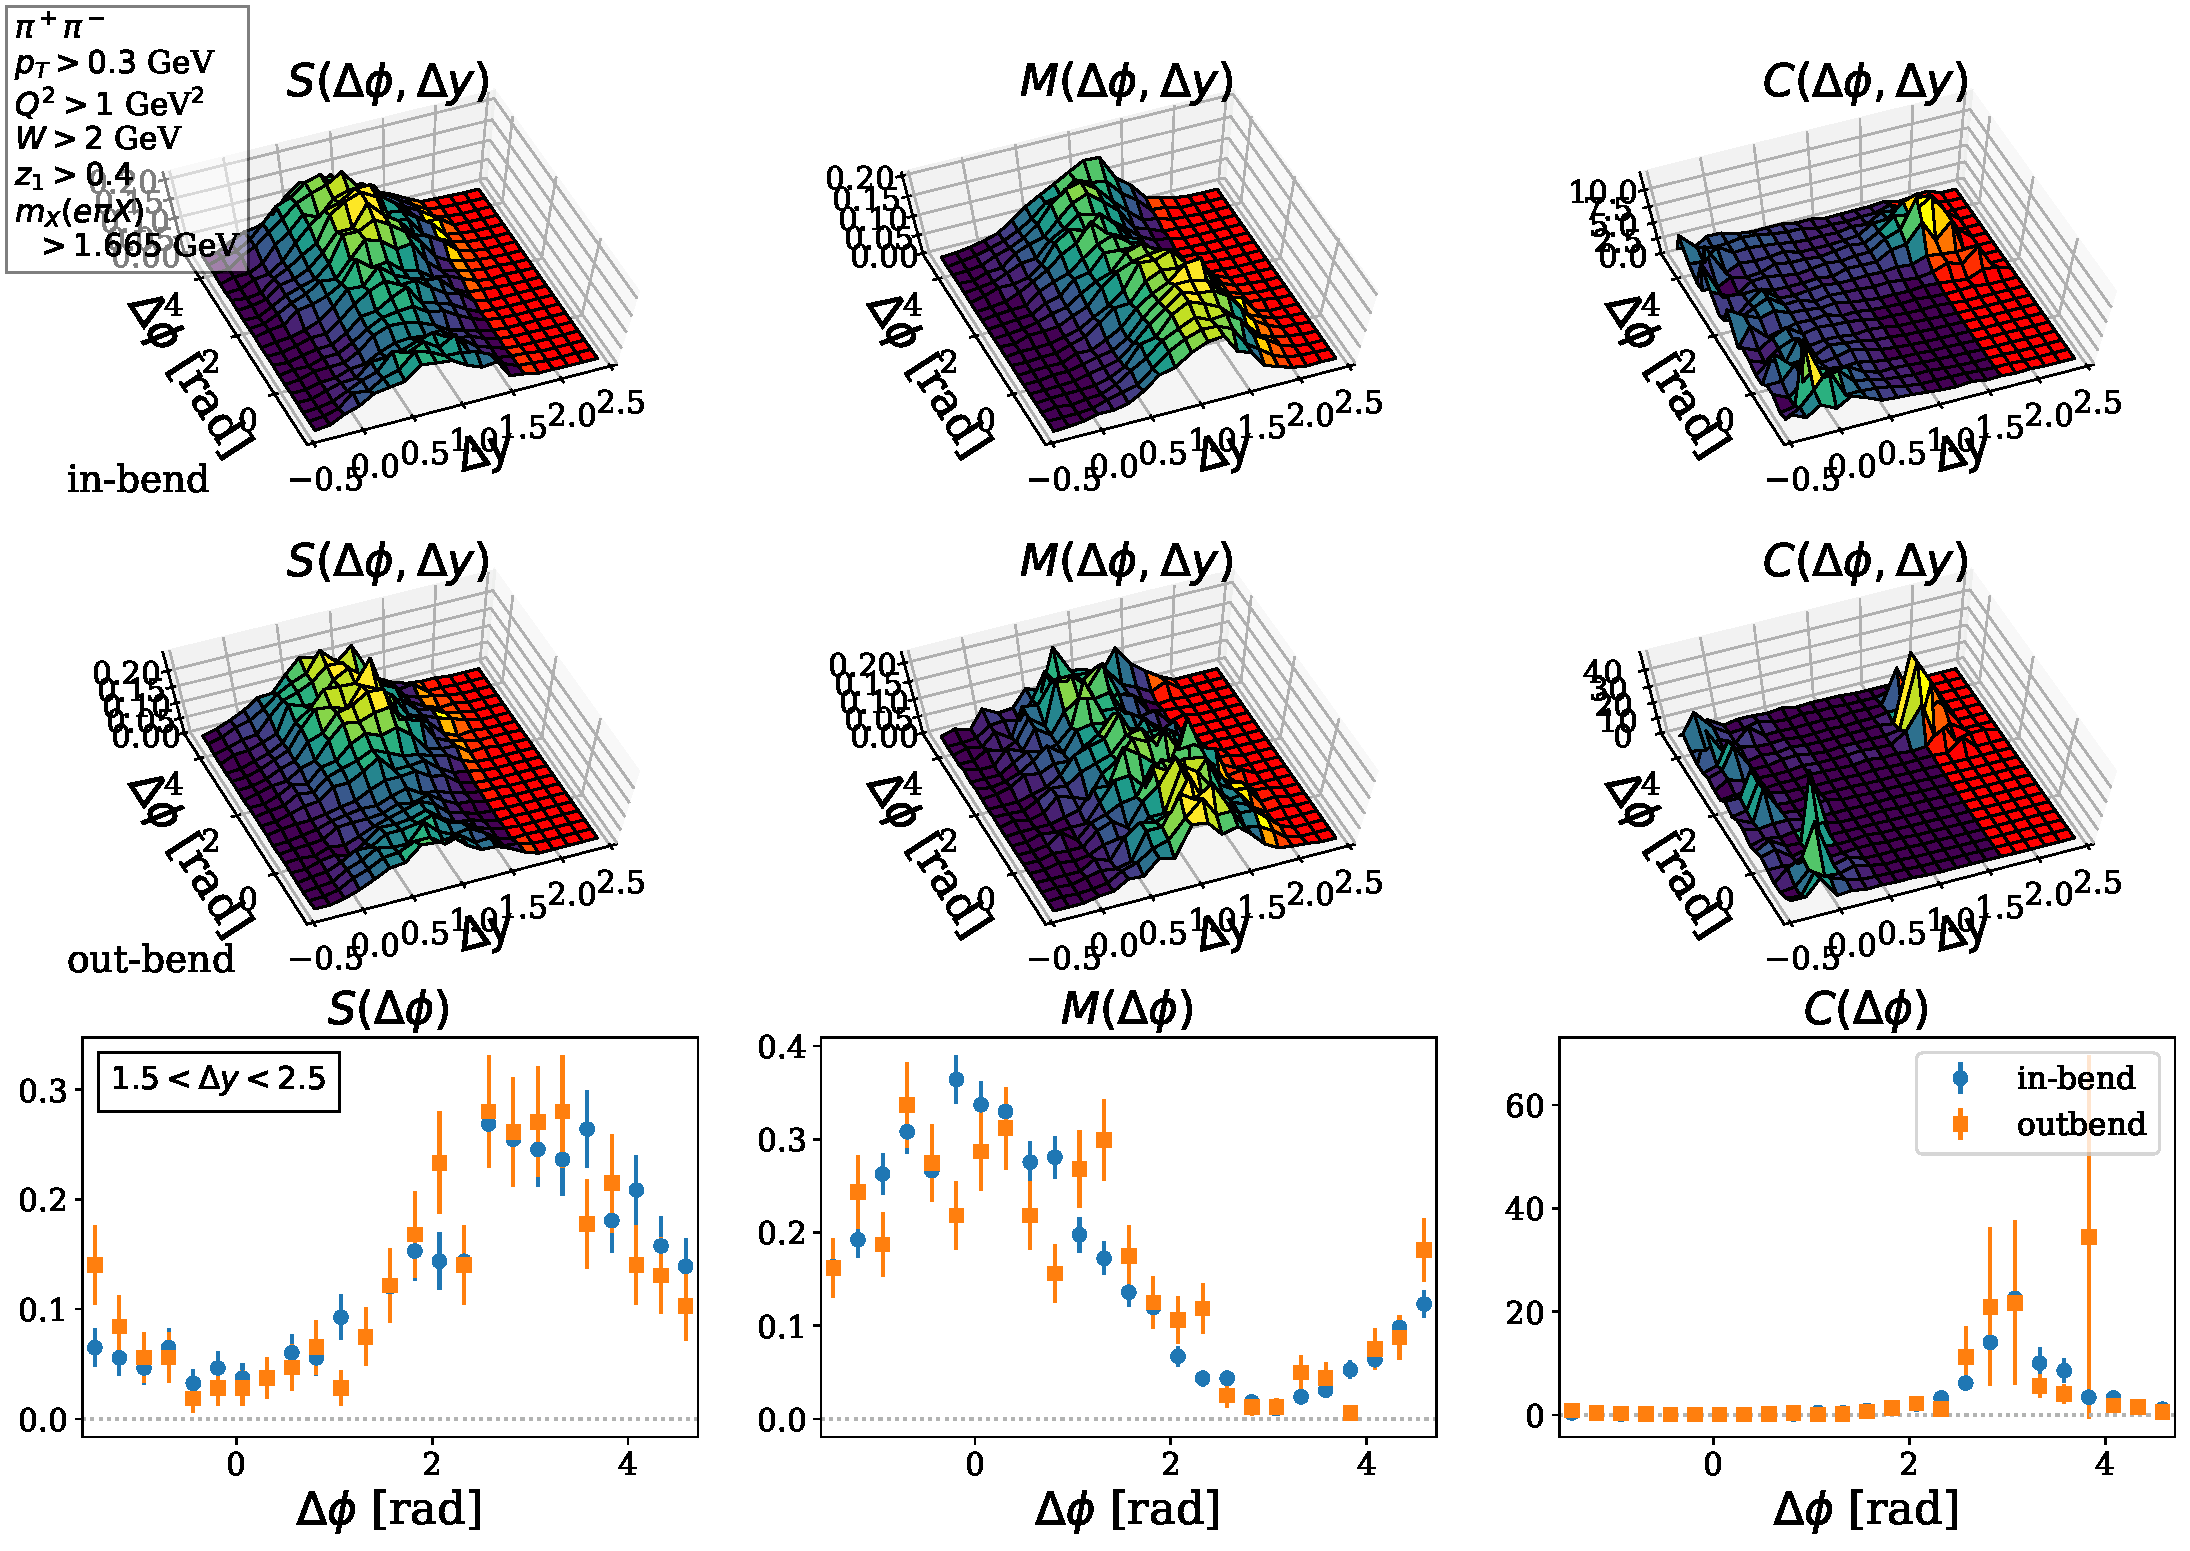
\includegraphics[width=\textwidth]{images/smc_inout_pi+pi-.pdf}
    \caption{Same as Fig.~\ref{fig:smc_inout_pi+p} for $\pi^+\pi^-$}
    \label{fig:smc_inout_pi+pi-}
\end{figure}

\begin{figure}
    \centering
    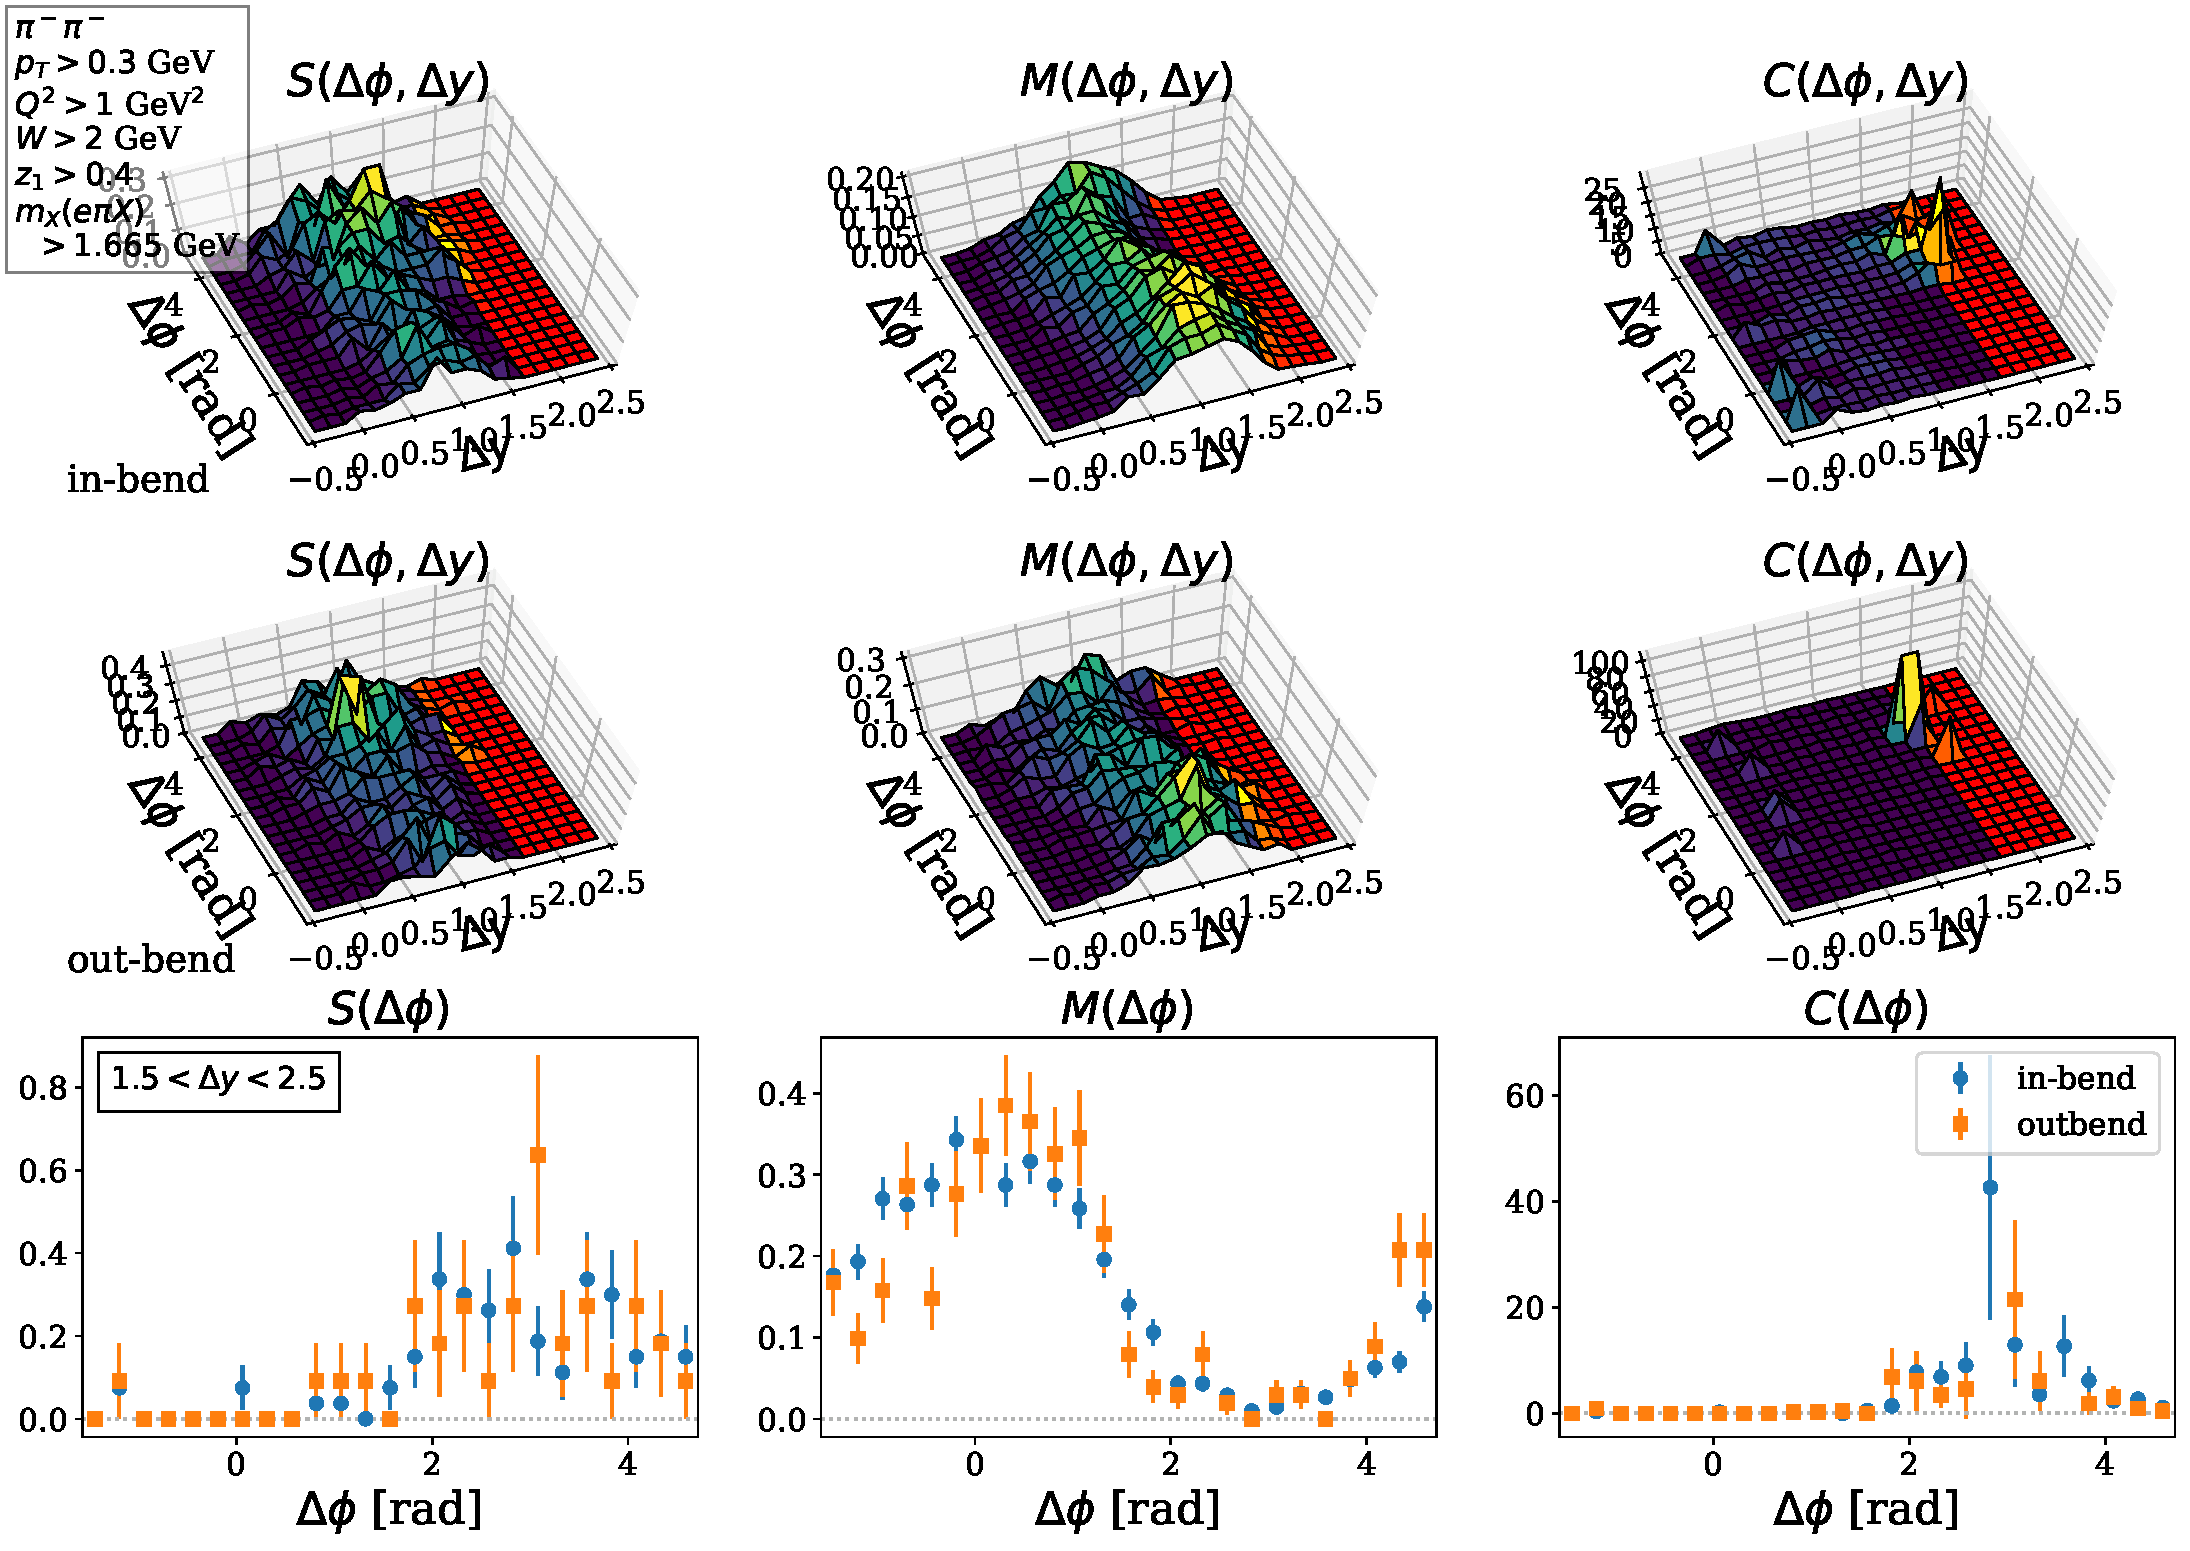
\includegraphics[width=\textwidth]{images/smc_inout_pi-pi-.pdf}
    \caption{Same as Fig.~\ref{fig:smc_inout_pi+p} for $\pi^-\pi^-$}
    \label{fig:smc_inout_pi-pi-}
\end{figure}

\subsection{Validation of the event-mixing procedure}
To validate the event mixing procedure, we plot in Fig.~\ref{fig:mix_test} (from left to right)  the probability density distributions of the lab-frame azimuthal angles of the two hadrons $\phi^{\rm lab}_1$ and $\phi^{\rm lab}_2$, and their difference $\Delta\phi^{\rm lab}$ for the mixed event sample.  The two rows represent the $\pi p$ and $\pi\pi$ samples.  The purpose of using the lab-frame $\phi$ is to have a variable that is independent of the underlying physics.  We also plot, in the right-most column, the following quantity:
\begin{equation}
\label{{eq:p_expected}
    P_{\rm expected}(\Delta\phi)= \int d\phi^{lab}_1 P(\phi^{\rm lab}_1) P(\phi^{\rm lab}_1-\Delta\phi^{\rm lab}) 
\end{equation}

where $P(...)$ represents the probability-density function for the enclosed quantity.  

\begin{figure}
    \centering
    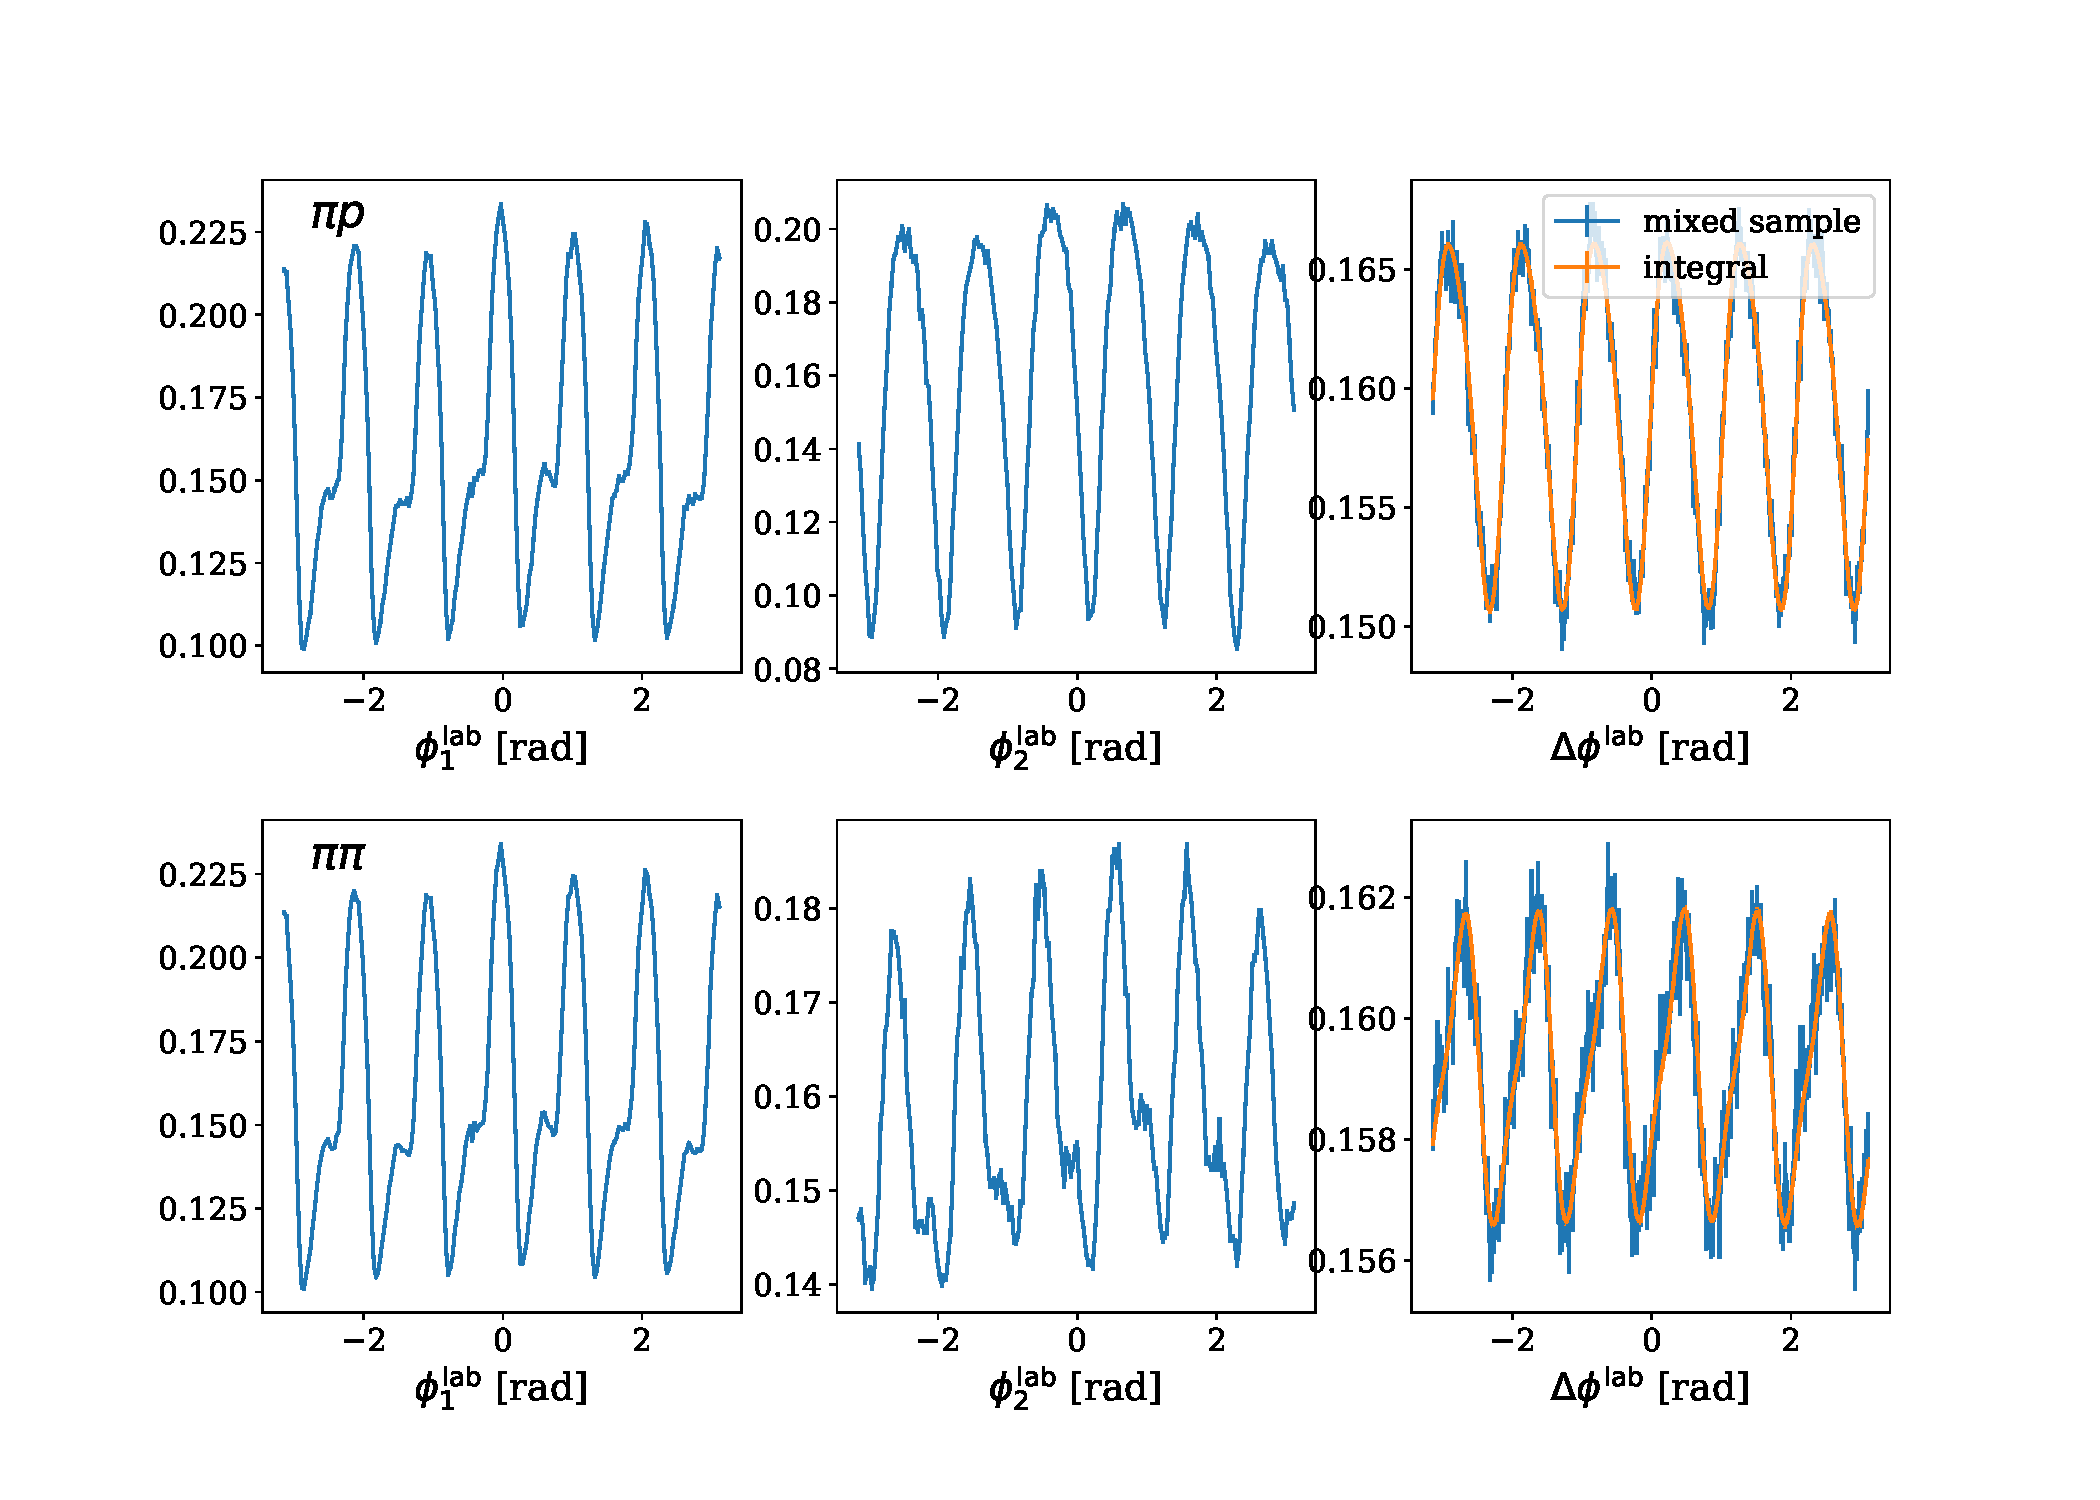
\includegraphics[width=\textwidth]{images/mix_test_concat.pdf}
    \caption{The probability density distributions of the lab-frame azimuthal angles of the trigger hadrons (left column) and associated hadrons (middle column), and their difference (right column, blue).  Also in the right column is the expected probability-density function for the difference (orange, see Eq.~\ref{eq:p_expected}}
    \label{fig:mix_test}
\end{figure}
